\clearpage
%
% PART III: Special Benchmarks
%
% Make listings font size smaller for input and output files
\lstset{basicstyle=\ttfamily\scriptsize, columns=fullflexible, keepspaces=true}
%
% QUESTION 1
%
\subsection{Clamped Beam with Nodal Load, Influence of Shear Deformability}
\begin{figure}[h]
    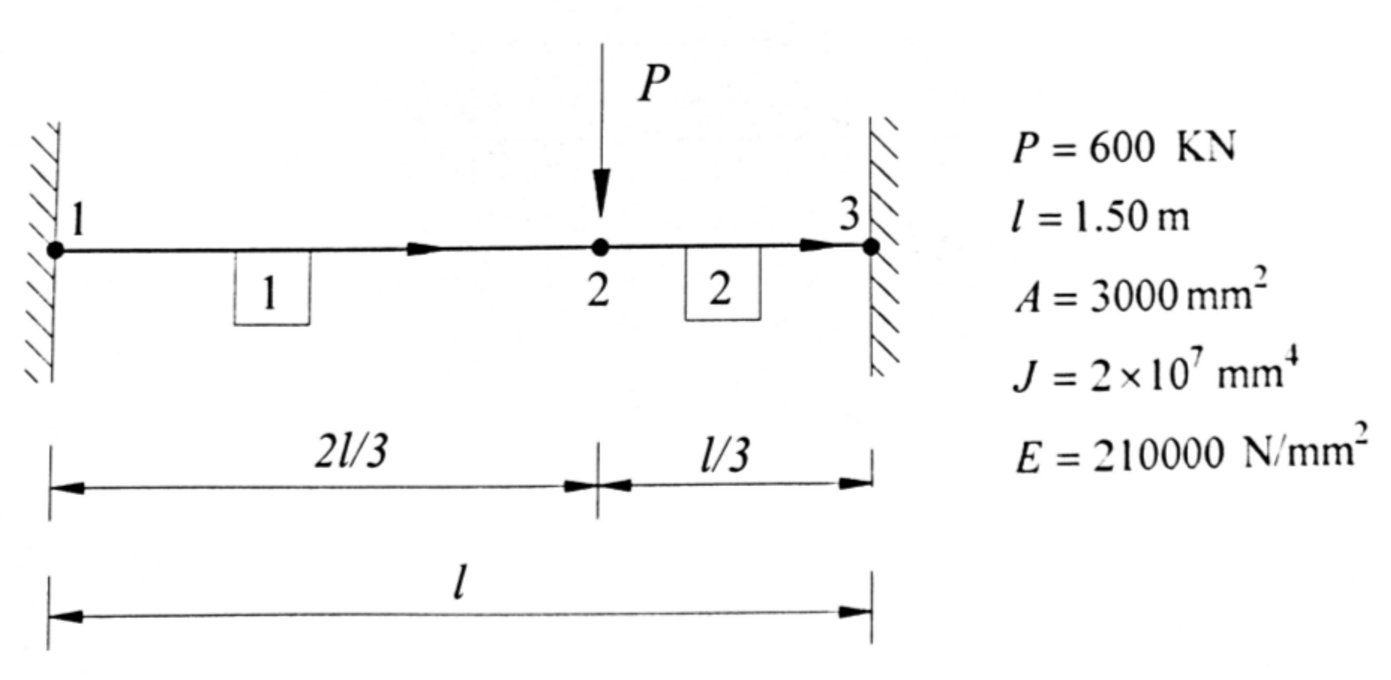
\includegraphics[scale=0.60]{%
                            bm_figures/turtle_figures/bmsp01_turtle.pdf}
    \centering
    \caption{Specialized Problem 1: Loading, geometry and supports}
    \label{fig:bmsp01_turtle}
\end{figure}
%
% Without shear deformability
%
\subsubsection{Without Shear Deformability}
\lstinputlisting{input_files/bmsp01_noshear_input.dat}
\lstinputlisting{output_files/bmsp01_noshear_output.dat}
% Deformed
\begin{figure}[!htb]
    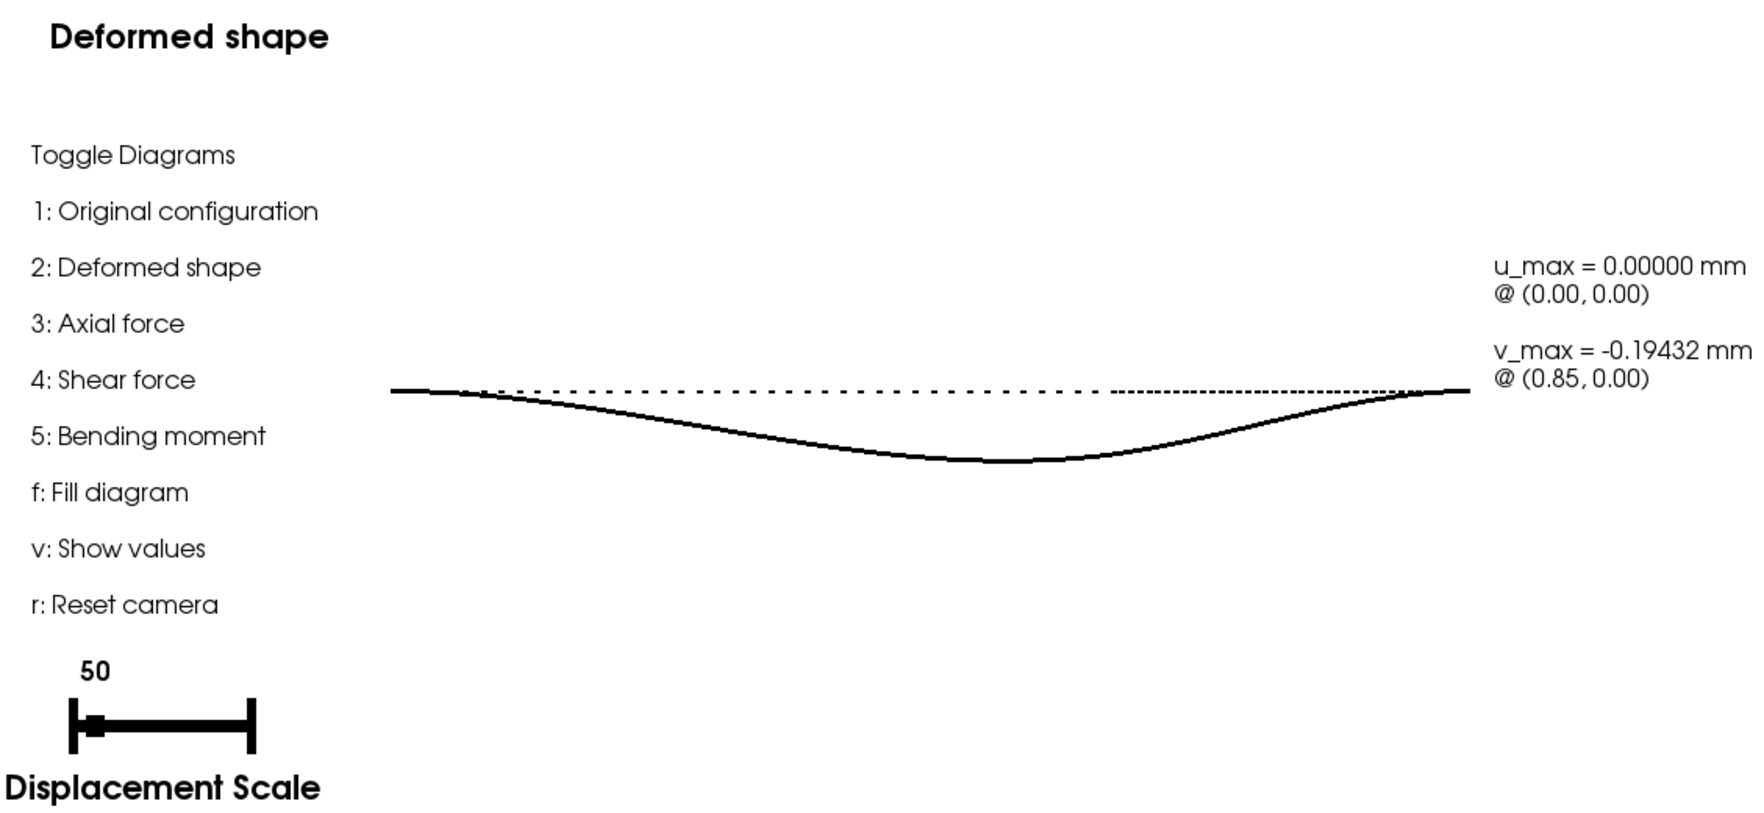
\includegraphics[width=\textwidth, keepaspectratio]{%
                     bm_figures/vtk_figures/bmsp01_noshear_deformed.pdf}
    \centering
    \caption{Specialized Problem 1: Deformed Shape (without shear deformability)}
    \label{fig:bmsp01_noshear_deformed}
\end{figure}
% Shear
\begin{figure}[!htb]
    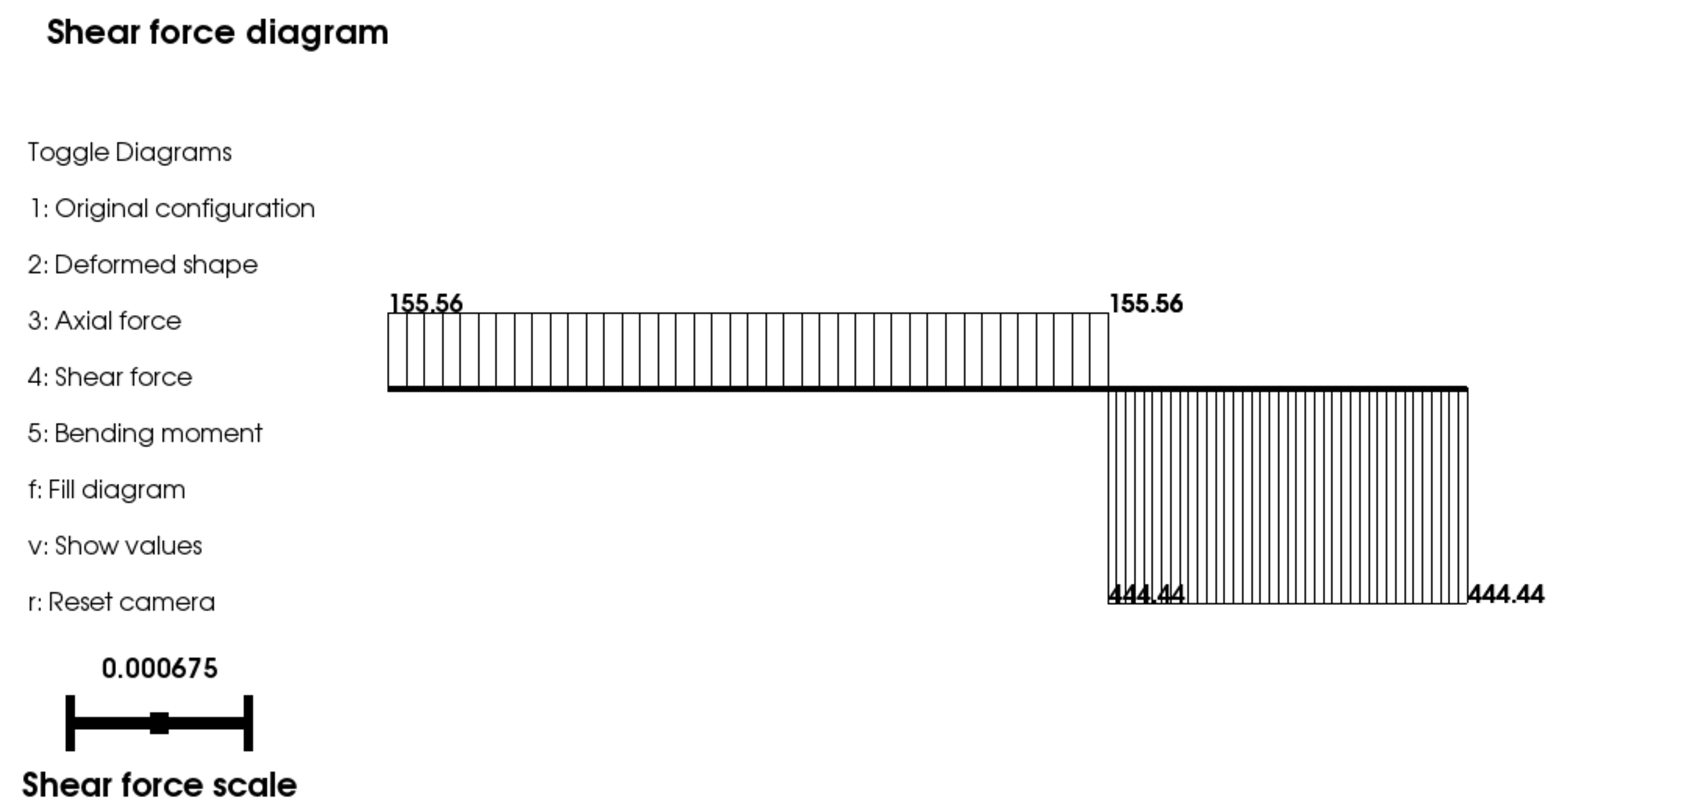
\includegraphics[width=\textwidth, keepaspectratio]{%
                     bm_figures/vtk_figures/bmsp01_noshear_shear.pdf}
    \centering
    \caption{Specialized Problem 1: Shear Force Diagram (without shear deformability)}
    \label{fig:bmsp01_noshear_shear}
\end{figure}
% Moment
\begin{figure}[!htb]
    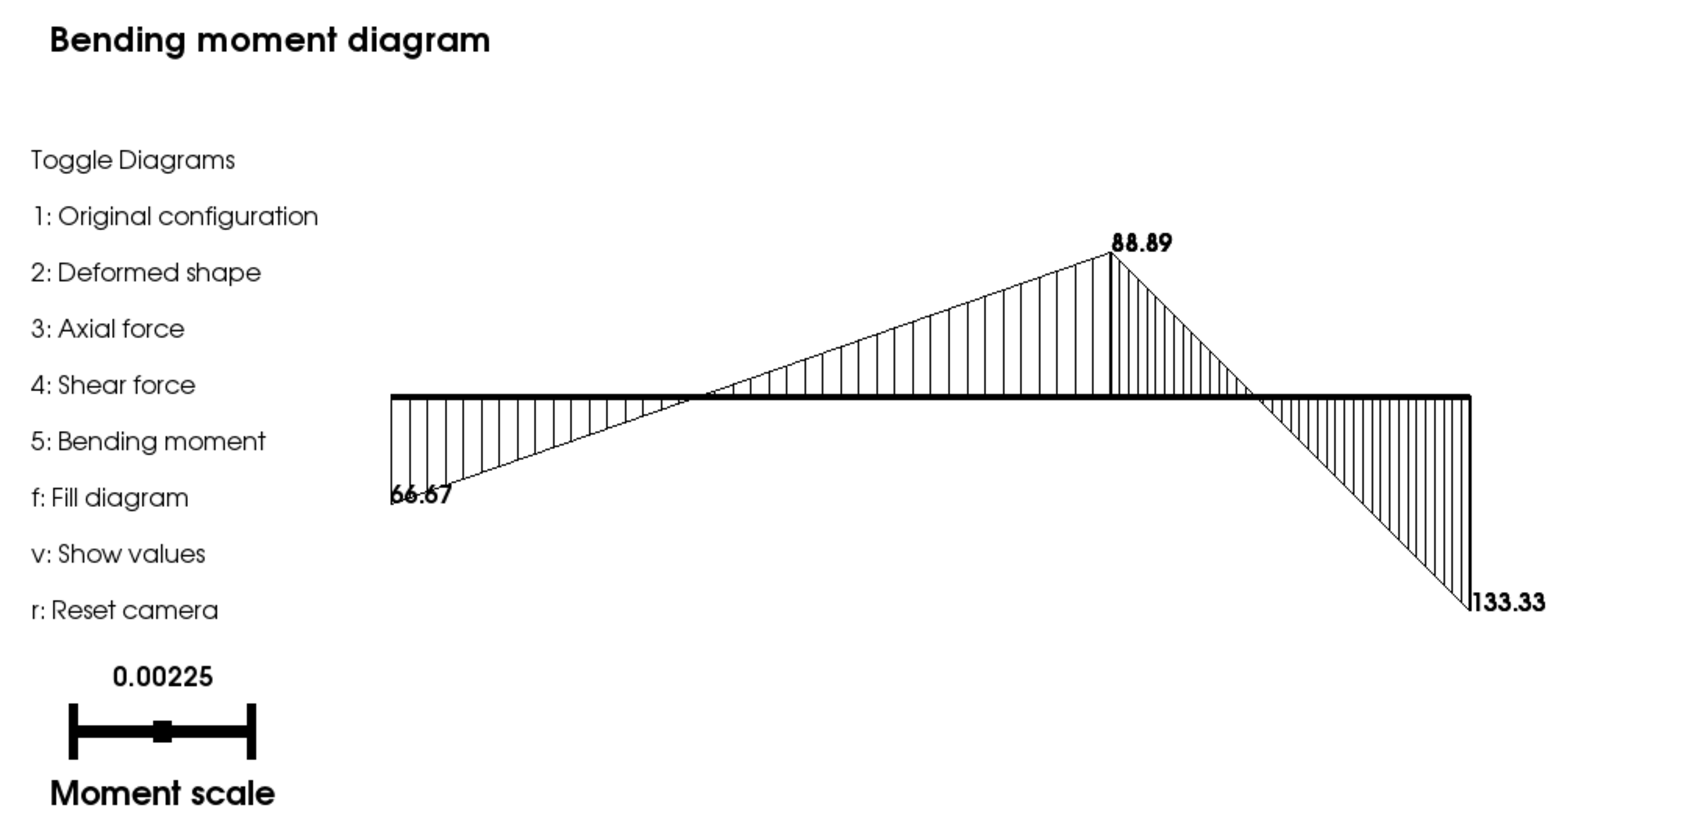
\includegraphics[width=\textwidth, keepaspectratio]{%
                     bm_figures/vtk_figures/bmsp01_noshear_moment.pdf}
    \centering
    \caption{Specialized Problem 1: Bending Moment Diagram (without shear deformability)}
    \label{fig:bmsp01_noshear_moment}
\end{figure}
% Error
\begin{table}[h!]
\centering
\begin{tabular}{ c| c c c c }
    & Exact Expression & Exact Value & Computed Value & \% RE \\ \hline \\
    $v_B$  & $-\dfrac{P(\dfrac{2}{3}l)^3(\dfrac{1}{3}l)^3}{3EJl^3}$ & -0.17637E-02 & -0.17637E-02 & 0.0\% \\ \\
    $\varphi_B$ & $-\dfrac{P(\dfrac{2}{3}l)^2(\dfrac{1}{3}l)^3}{2EJl^3}$ & 0.26455E-02 & 0.26455E-02 & 0.0\% \\ \\
\end{tabular}
\end{table}
%
% With shear deformability
%
\subsubsection{With Shear Deformability}
\par
Shear deformability is introduced by setting $\chi=2.5$ and $\nu=0.3$, while all other parameters 
were held constant. The results are presented below.
\lstinputlisting{input_files/bmsp01_wshear_input.dat}
\lstinputlisting{output_files/bmsp01_wshear_output.dat}
% Deformed
\begin{figure}[!htb]
    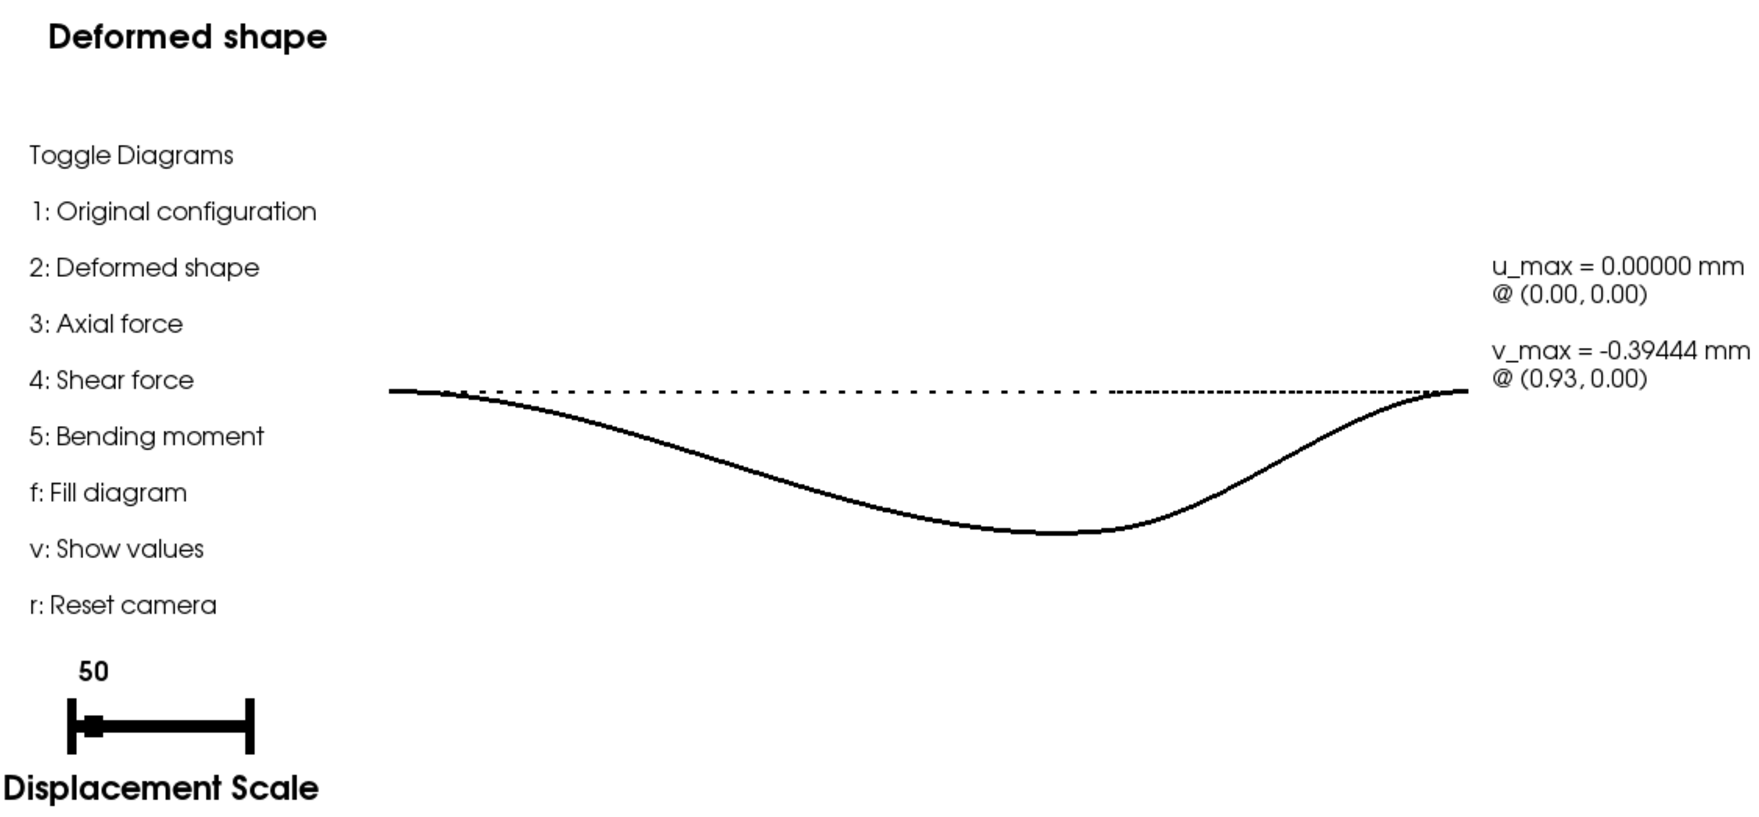
\includegraphics[width=\textwidth, keepaspectratio]{%
                     bm_figures/vtk_figures/bmsp01_wshear_deformed.pdf}
    \centering
    \caption{Specialized Problem 1: Deformed Shape (with shear deformability)}
    \label{fig:bmsp01_wshear_deformed}
\end{figure}
% Shear
\begin{figure}[!htb]
    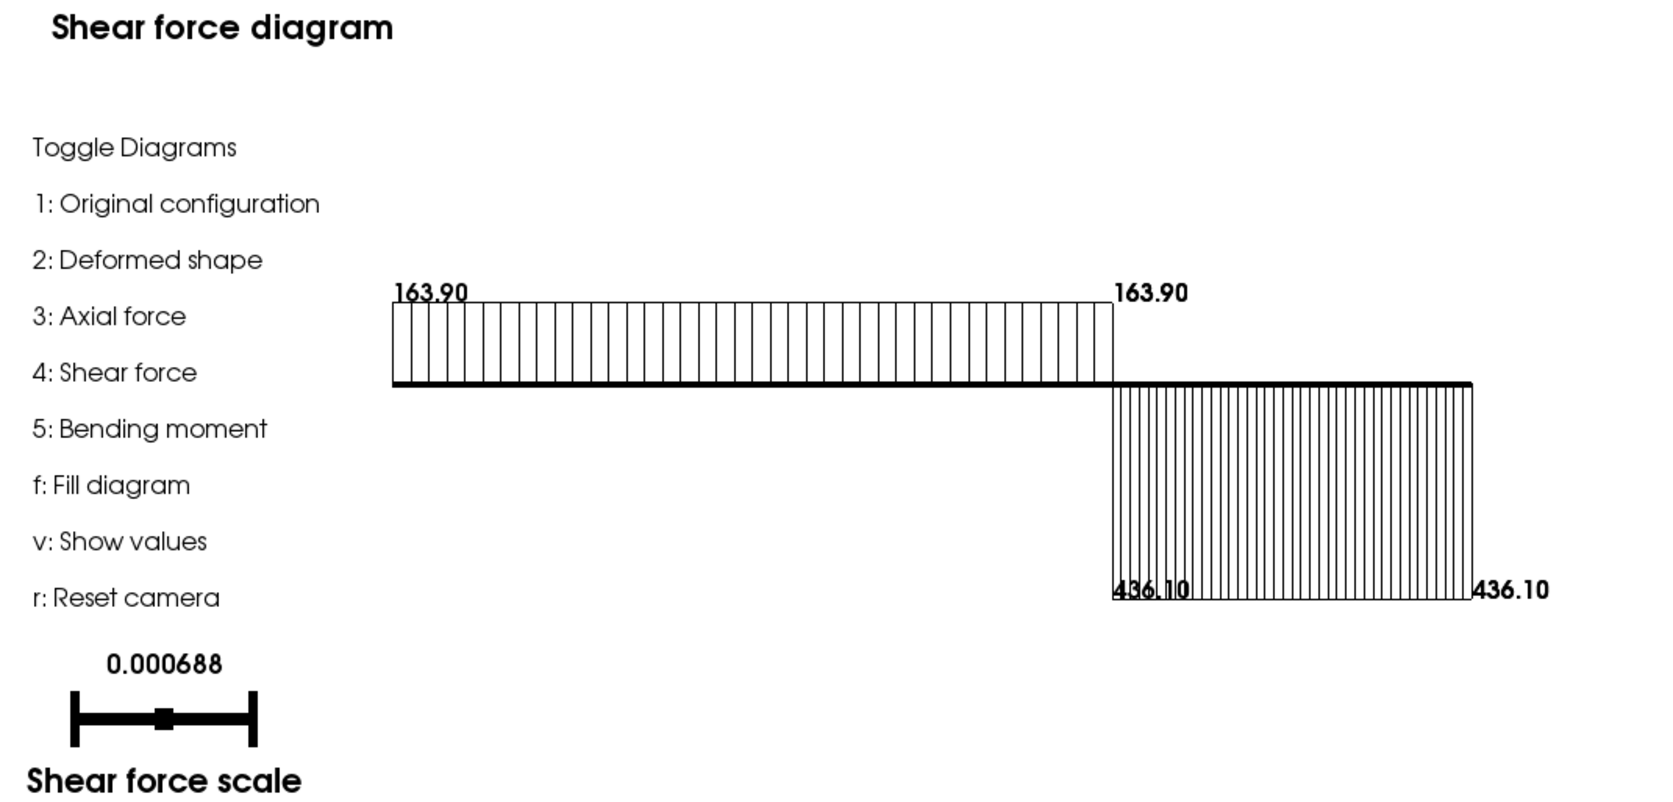
\includegraphics[width=\textwidth, keepaspectratio]{%
                     bm_figures/vtk_figures/bmsp01_wshear_shear.pdf}
    \centering
    \caption{Specialized Problem 1: Shear Force Diagram (with shear deformability)}
    \label{fig:bmsp01_wshear_shear}
\end{figure}
% Moment
\begin{figure}[!htb]
    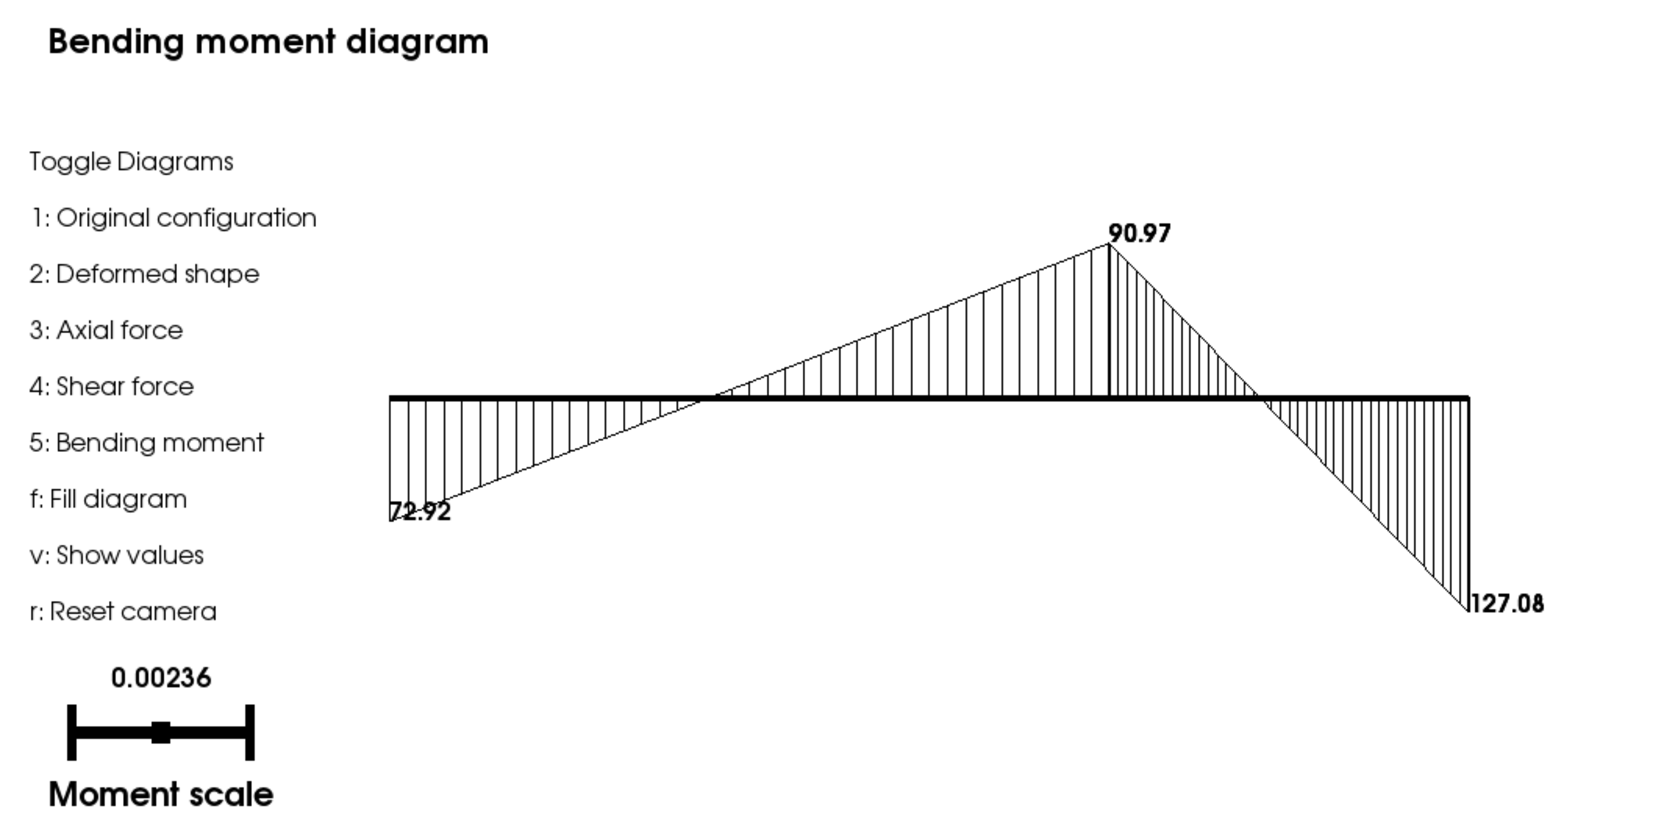
\includegraphics[width=\textwidth, keepaspectratio]{%
                     bm_figures/vtk_figures/bmsp01_wshear_moment.pdf}
    \centering
    \caption{Specialized Problem 1: Bending Moment Diagram (with shear deformability)}
    \label{fig:bmsp01_wshear_moment}
\end{figure}
% Error
\begin{table}[h!]
\centering
\begin{tabular}{ c| c c c }
    & Exact Value & Computed Value & \% RE \\ \hline \\
    $v_B$  & -0.3869E-02 & -0.3869E-02 & 0.0\% \\ \\
    $\phi_B$ & 0.2149E-02 & 0.2149E-02 & 0.0\% \\ \\
\end{tabular}
\end{table}
% Comments
\par
As can be observed from the presnted values, introducing shear deformability results in a 
significant variation in nodal displacement and rotation:
\begin{equation*}
    \dfrac{\delta v}{v_t} = \dfrac{v_t - v_m}{v_t} = %
        \dfrac{|-0.3869E-02 - (-0.1764E-02)|}{|-0.3869E-02|} = 54.4\% \\
    \dfrac{\delta \varphi}{\varphi_t} = \dfrac{\varphi_t - \varphi_m}{\varphi_t} = %
        \dfrac{|0.2149E-02 - 0.2646E-02|}{|0.2149E-02|} = 23.1\% 
\end{equation*}
\par
However, the variation in the internal force resultants are rather low when compared to that of the
displacements, for instance the variation in the moments at nodes 1 and 3:
\begin{equation*}
    \dfrac{\delta M_1}{M_{1,t}} = \dfrac{M_{1,t} - M_{1,m}}{M_{1,t}} = %
        \dfrac{|-0.72924E+02 - (-0.66667E+02)|}{|-0.72924E+02|} = 8.6\% \\
    \dfrac{\delta M_3}{M_{3,t}} = \dfrac{M_{3,t} - M_{3,m}}{M_{3,t}} = %
        \dfrac{|-0.12708E+03 - (-0.13333E+03)|}{|-0.12708E+03|} = 4.9\% \\
\end{equation*}

%
% QUESTION 2  --- TODO ASK THE DEPTH OF THE CROSS SECTION TODO ---
%

%
% QUESTION 3
%
\subsection{Frame with Elastic Restraints and Linear Differential Temperature Change}
\begin{figure}[h]
    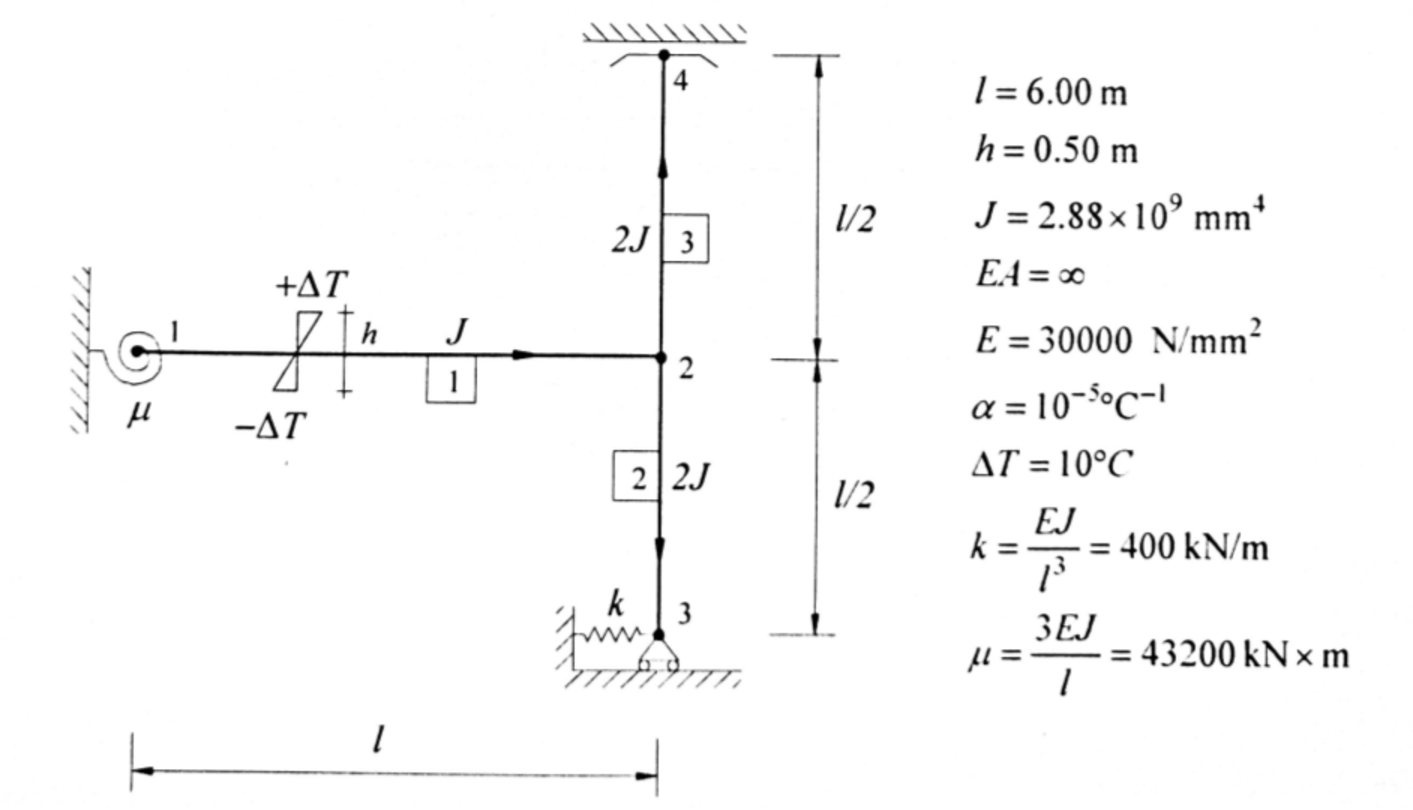
\includegraphics[scale=0.60]{%
                            bm_figures/turtle_figures/bmsp03_turtle.pdf}
    \centering
    \caption{Specialized Problem 3: Loading, geometry and supports}
    \label{fig:bmsp01_turtle}
\end{figure}
\lstinputlisting{input_files/bmsp03_input.dat}
\lstinputlisting{output_files/bmsp03_output.dat}
% Deformed
\begin{figure}[!htb]
    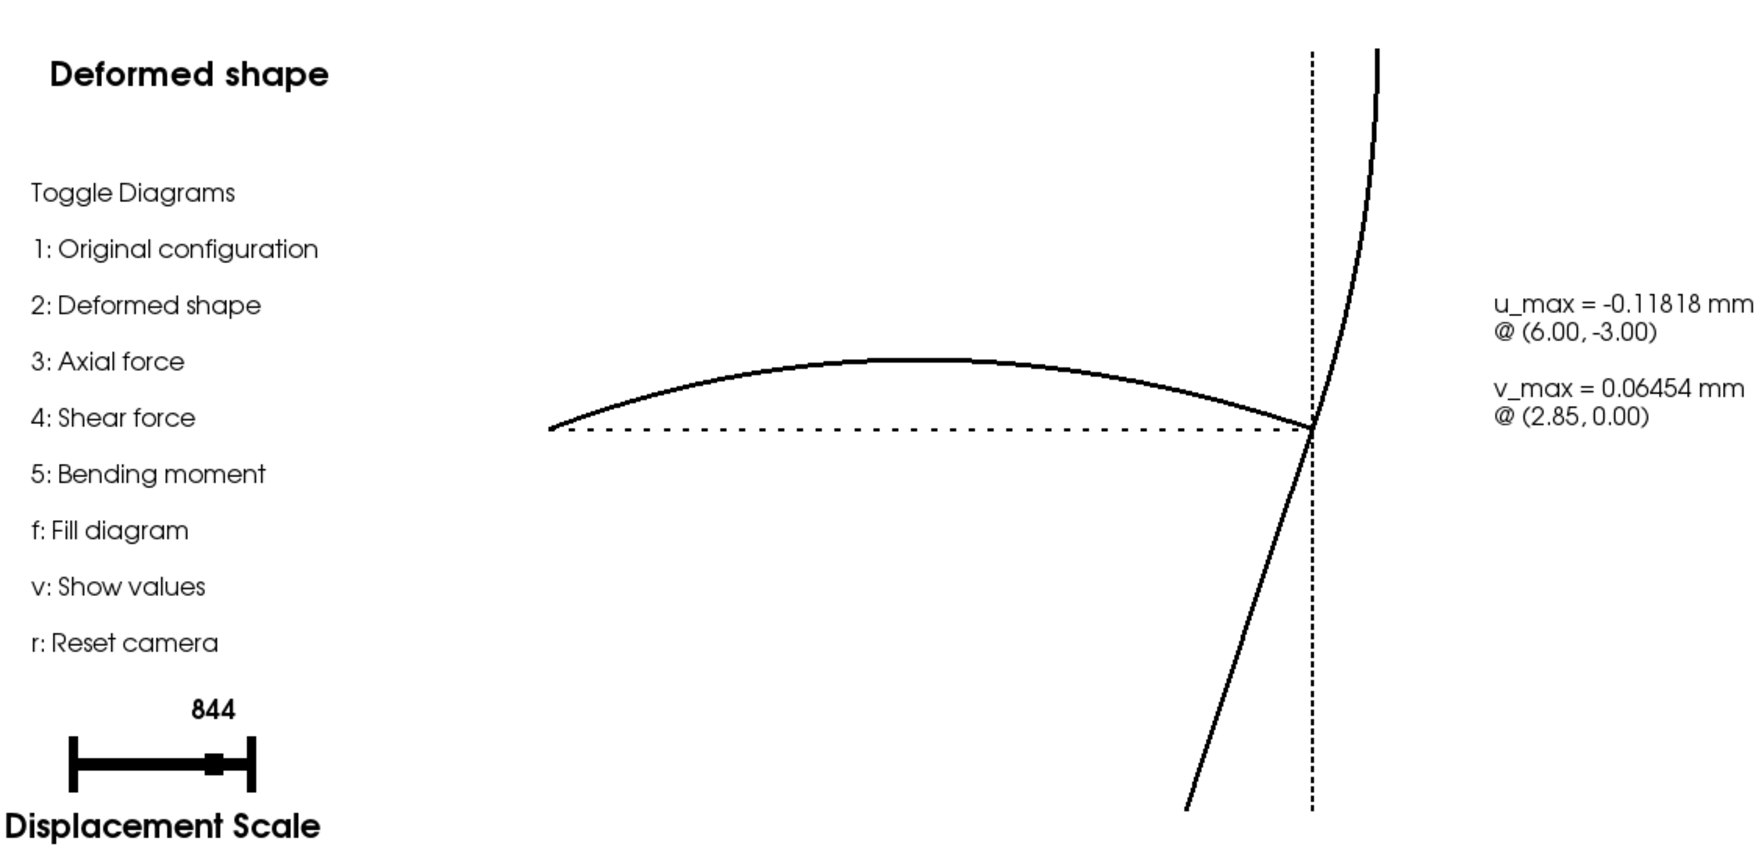
\includegraphics[width=\textwidth, keepaspectratio]{%
                     bm_figures/vtk_figures/bmsp03_deformed.pdf}
    \centering
    \caption{Specialized Problem 3: Deformed Shape}
    \label{fig:bmsp03_deformed}
\end{figure}
% Axial
\begin{figure}[!htb]
    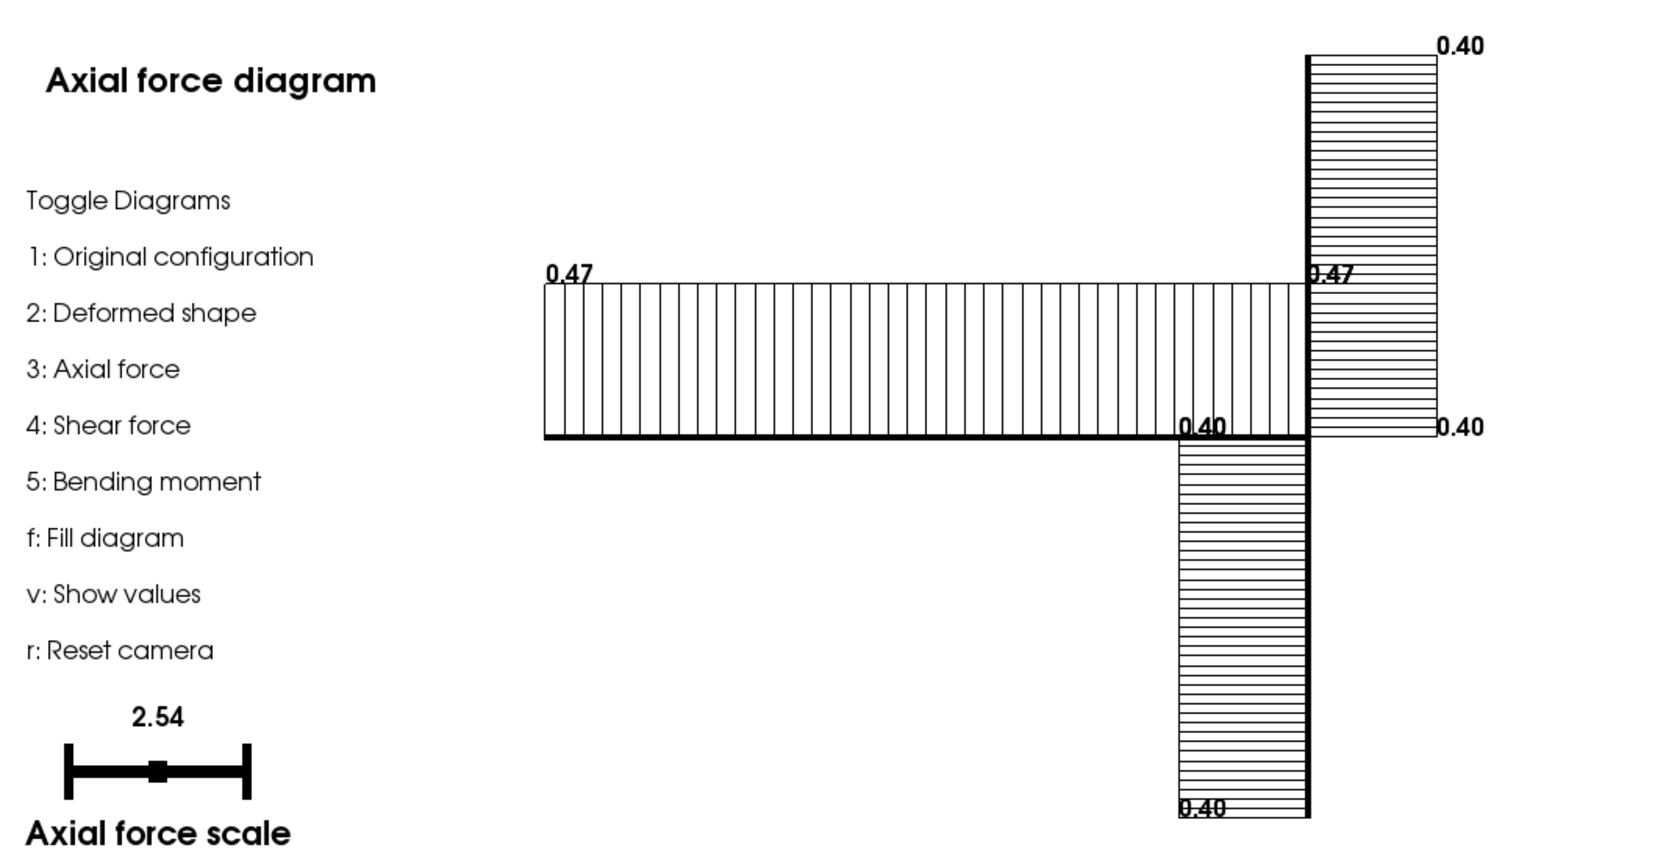
\includegraphics[width=\textwidth, keepaspectratio]{%
                     bm_figures/vtk_figures/bmsp03_axial.pdf}
    \centering
    \caption{Specialized Problem 3: Axial Force Diagram}
    \label{fig:bmsp03_shear}
\end{figure}

% Shear
\begin{figure}[!htb]
    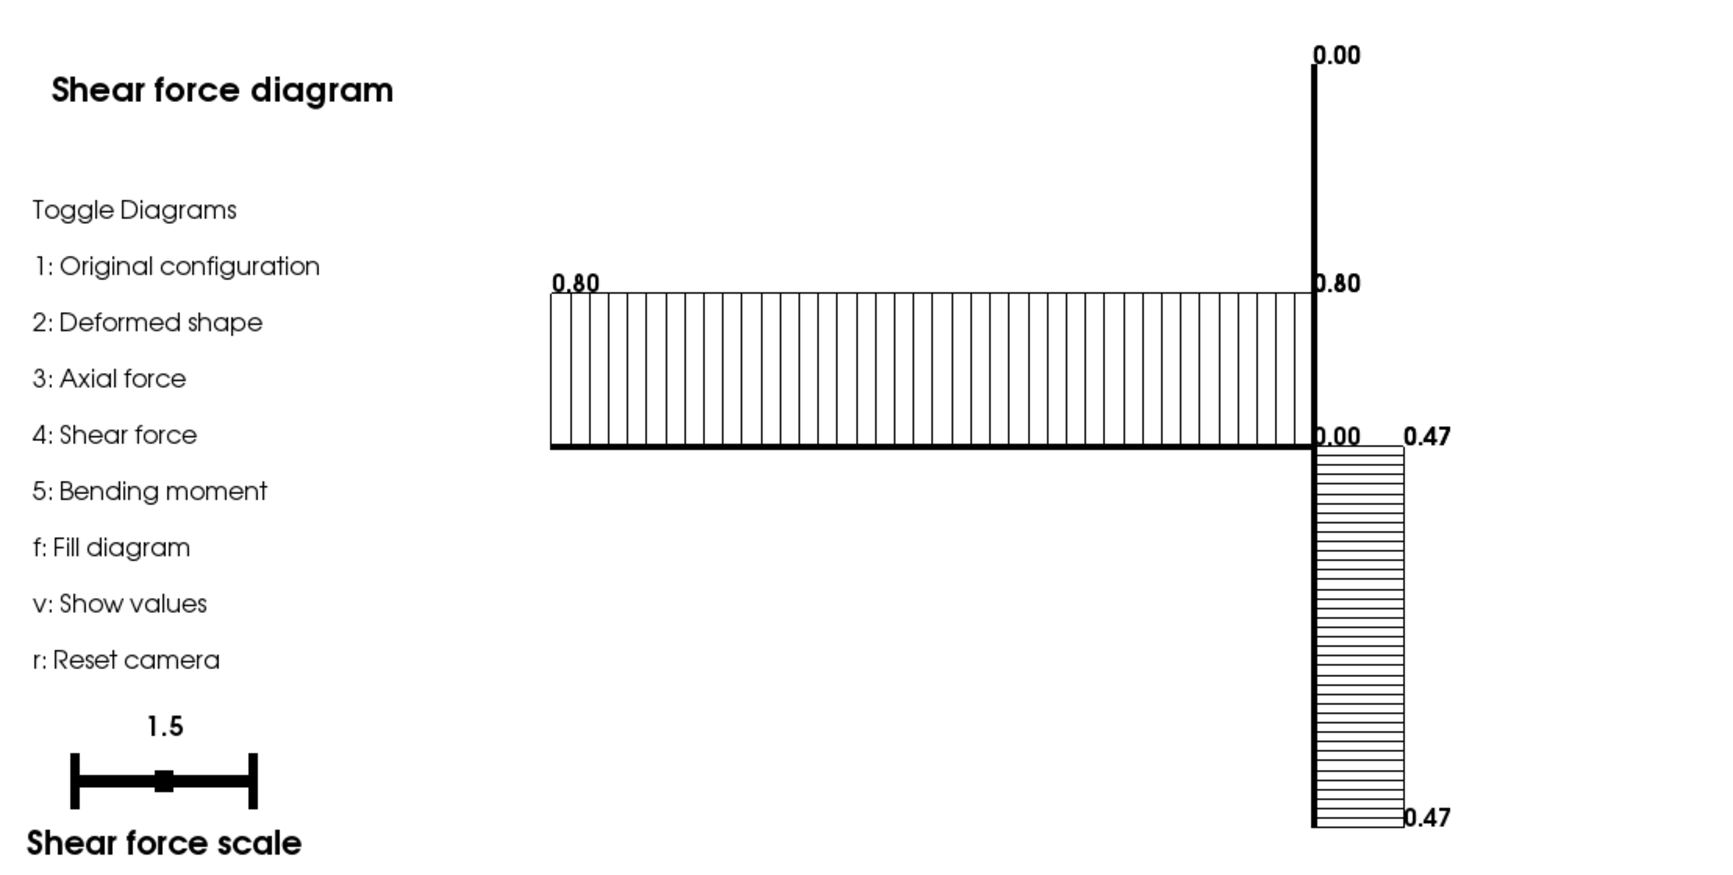
\includegraphics[width=\textwidth, keepaspectratio]{%
                     bm_figures/vtk_figures/bmsp03_shear.pdf}
    \centering
    \caption{Specialized Problem 3: Shear Force Diagram}
    \label{fig:bmsp03_shear}
\end{figure}
% Moment
\begin{figure}[!htb]
    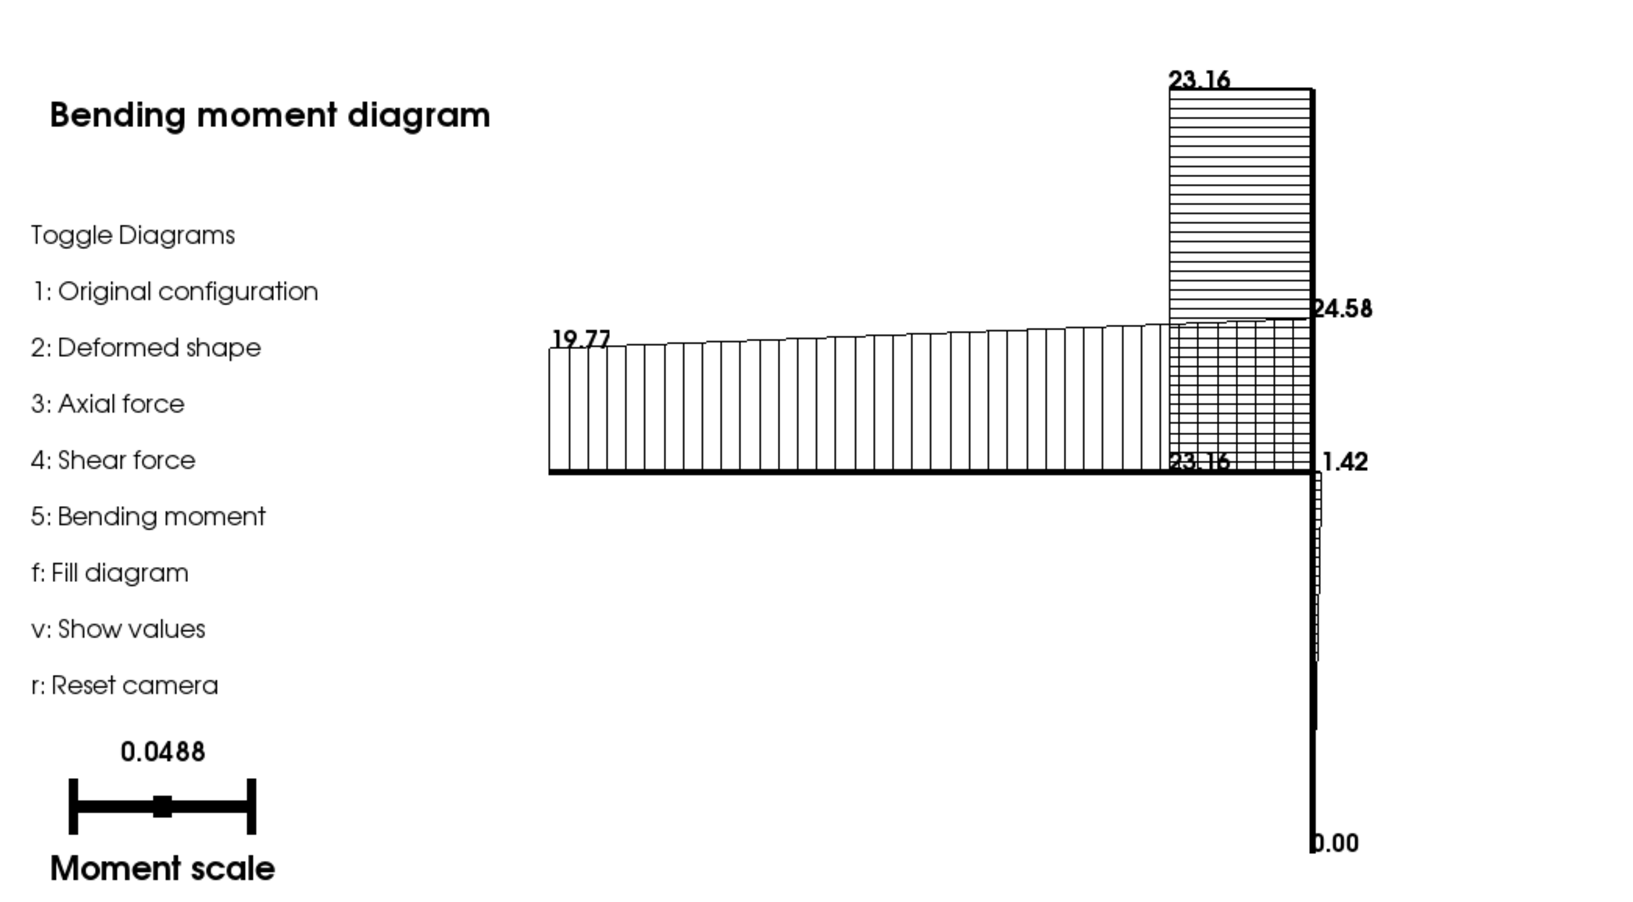
\includegraphics[width=\textwidth, keepaspectratio]{%
                     bm_figures/vtk_figures/bmsp03_moment.pdf}
    \centering
    \caption{Specialized Problem 3: Bending Moment Diagram}
    \label{fig:bmsp03_moment}
\end{figure}
% Error
\begin{table}[h!]
\centering
\begin{tabular}{ c| c c c }
    & Reference Value & Computed Value & \% RE \\ \hline \\
    $N_{23}=-N_{42}$  & 0.400E-00 & 0.400E-00 & 0.0\% \\ \\
    $N_{12}$          & 0.473E-00 & 0.473E-00 & 0.0\% \\ \\
    $T_{12}$          & 0.801E-00 & 0.801E-00 & 0.0\% \\ \\
    $T_{32}$          & -0.473E-00 & -0.473E-00 & 0.0\% \\ \\
    $M_{1}$           & -0.19775E+02 & 0.19775E-02 & 0.0\% \\ \\
    $M_{4}$           & 0.23163E-02 & 0.23163E-02 & 0.0\% \\ \\
    $\dfrac{\varphi_1}{|\varphi_2|}$ & 1.14 & 1.14 & 0.0\% \\ \\
\end{tabular}
\end{table}

%
% QUESTION 4
%
\subsection{Portal Frame with Inclined Roof Beams and Rod Ties}
\begin{figure}[h]
    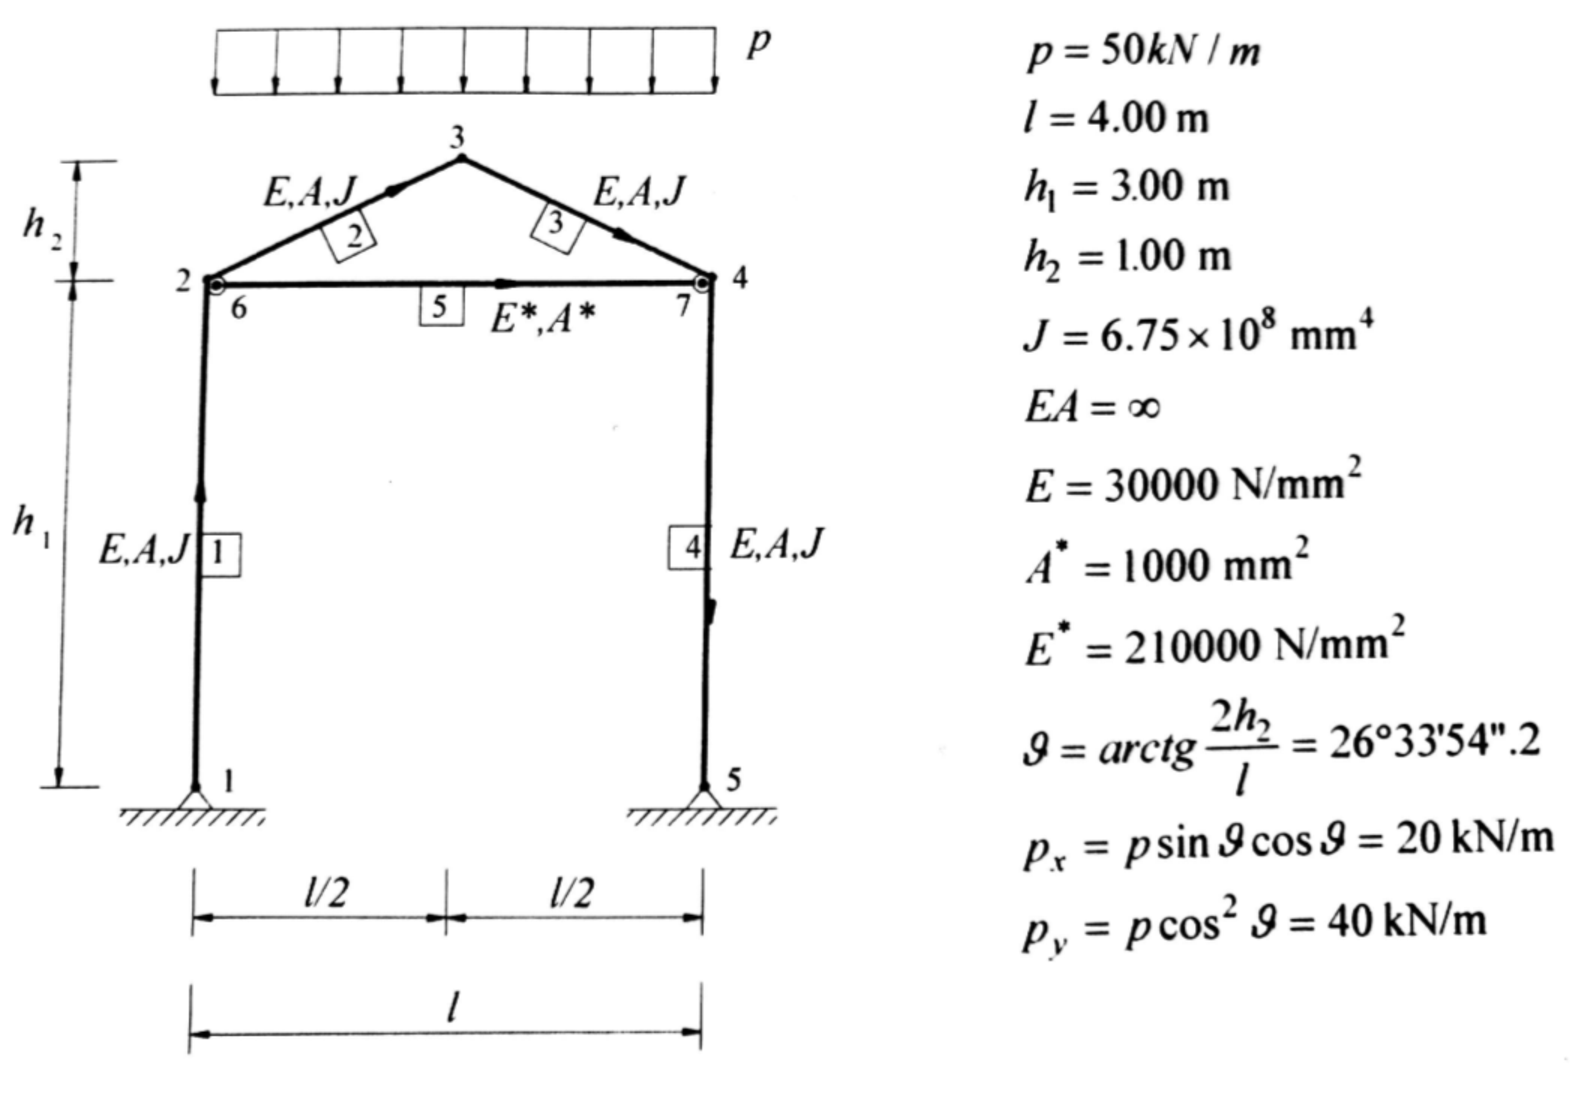
\includegraphics[scale=0.60]{%
                            bm_figures/turtle_figures/bmsp04_turtle.pdf}
    \centering
    \caption{Specialized Problem 4: Loading, geometry and supports}
    \label{fig:bmsp01_turtle}
\end{figure}
\lstinputlisting{input_files/bmsp04_input.dat}
\lstinputlisting{output_files/bmsp04_output.dat}
% Deformed
\begin{figure}[!htb]
    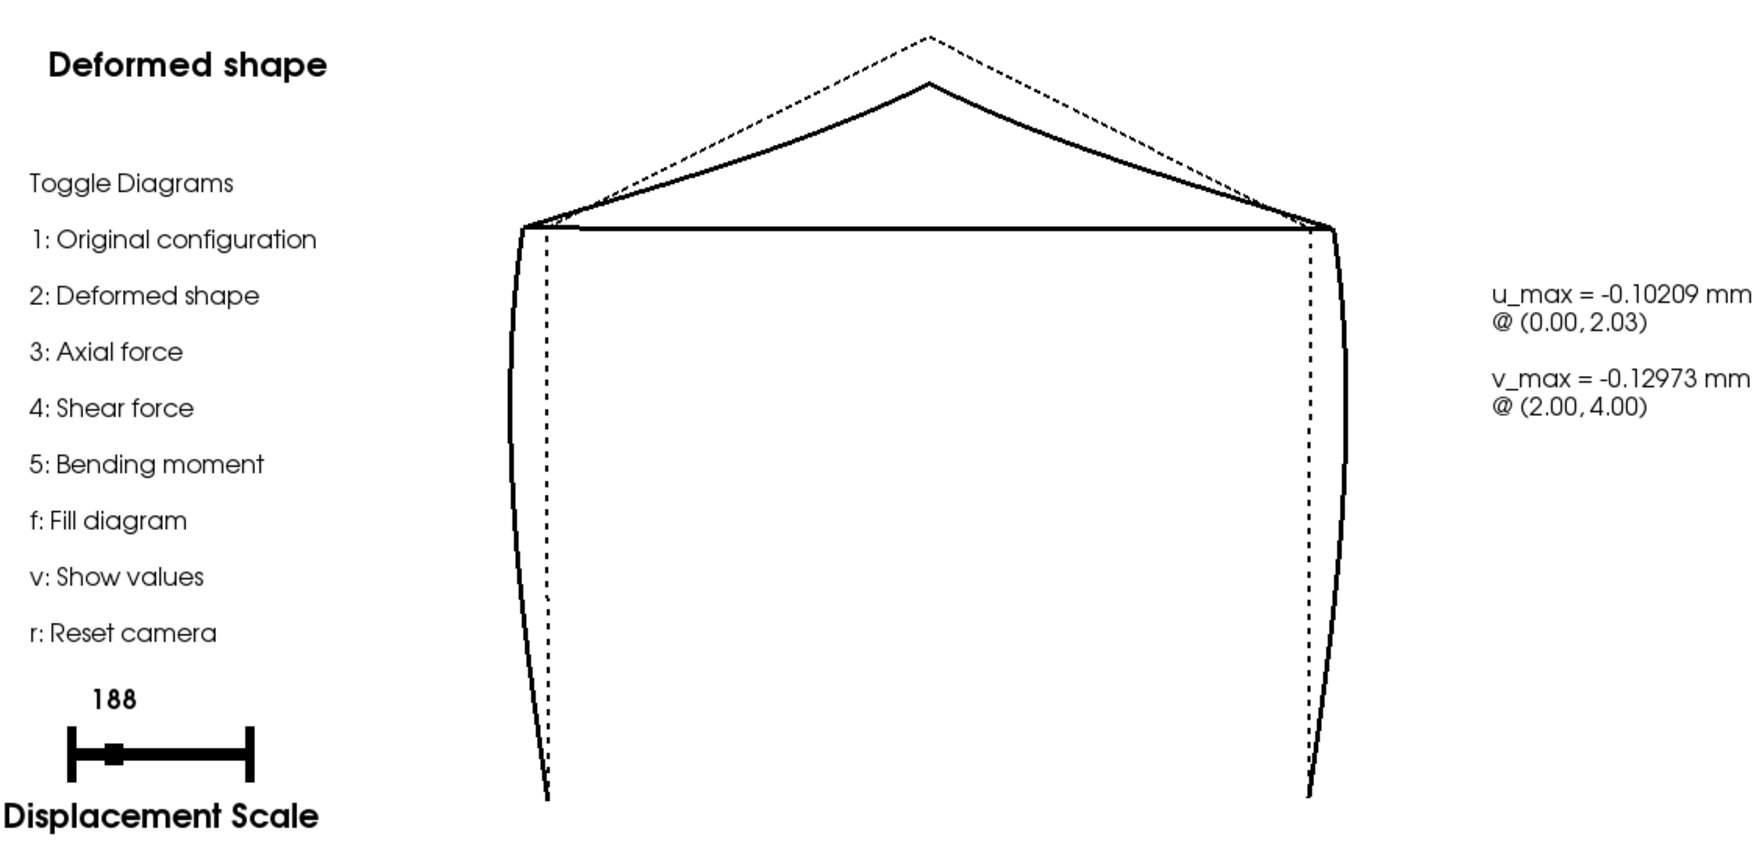
\includegraphics[width=\textwidth, keepaspectratio]{%
                     bm_figures/vtk_figures/bmsp04_deformed.pdf}
    \centering
    \caption{Specialized Problem 4: Deformed Shape}
    \label{fig:bmsp04_deformed}
\end{figure}
% Axial
\begin{figure}[!htb]
    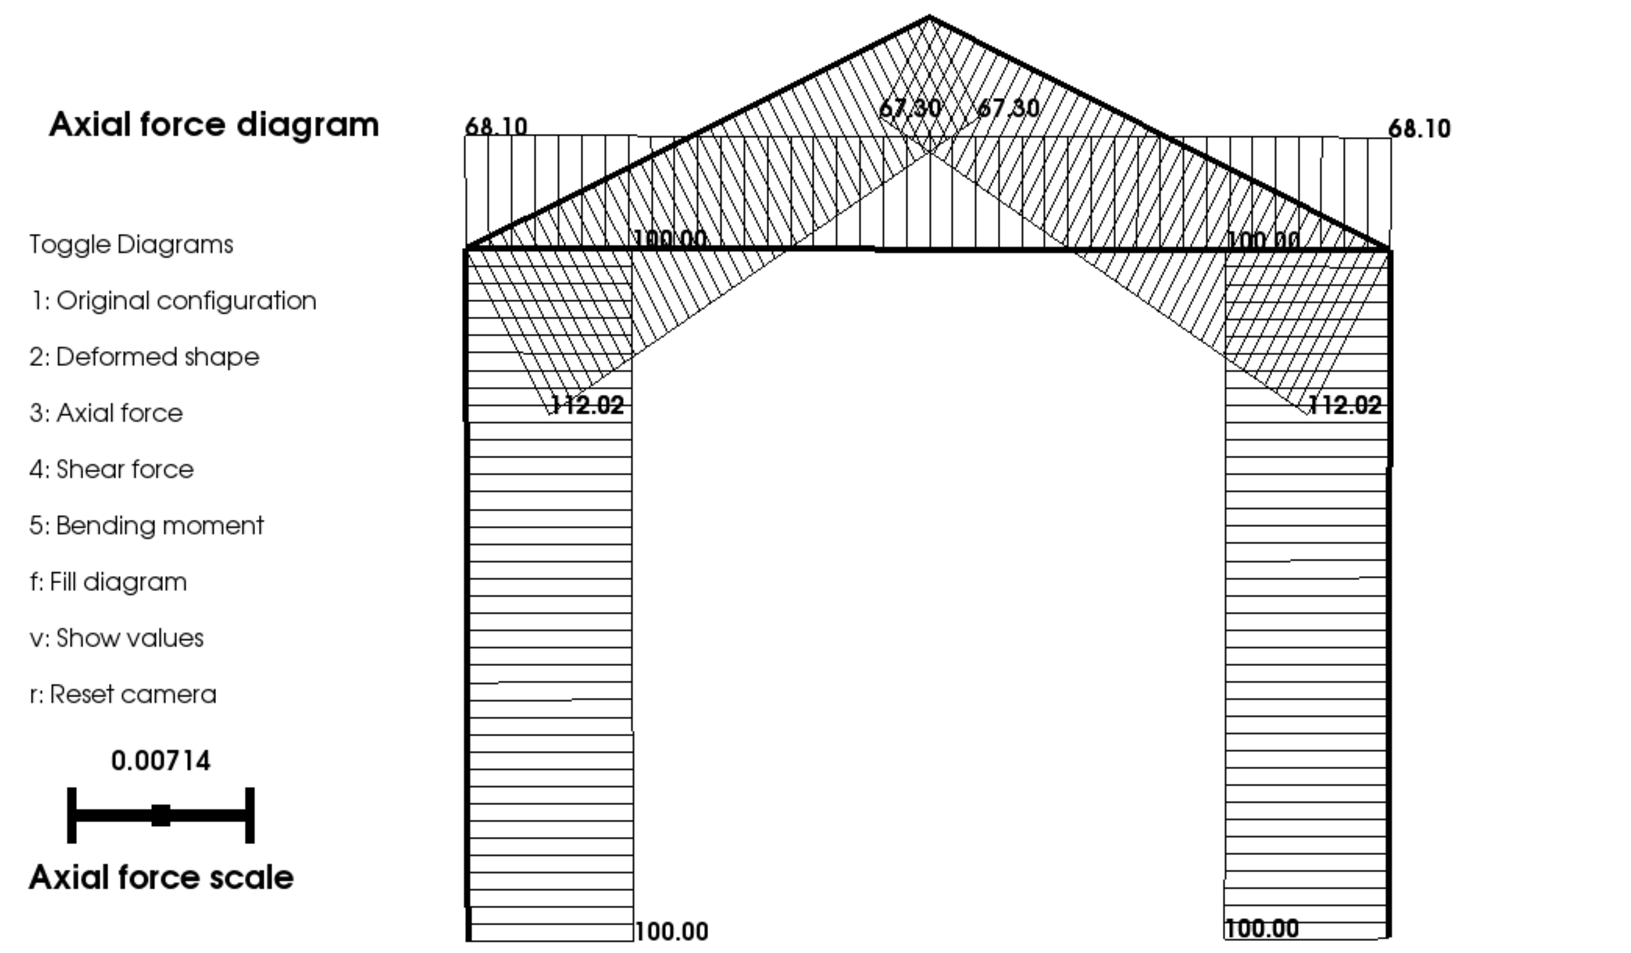
\includegraphics[width=\textwidth, keepaspectratio]{%
                     bm_figures/vtk_figures/bmsp04_axial.pdf}
    \centering
    \caption{Specialized Problem 4: Axial Force Diagram}
    \label{fig:bmsp04_shear}
\end{figure}

% Shear
\begin{figure}[!htb]
    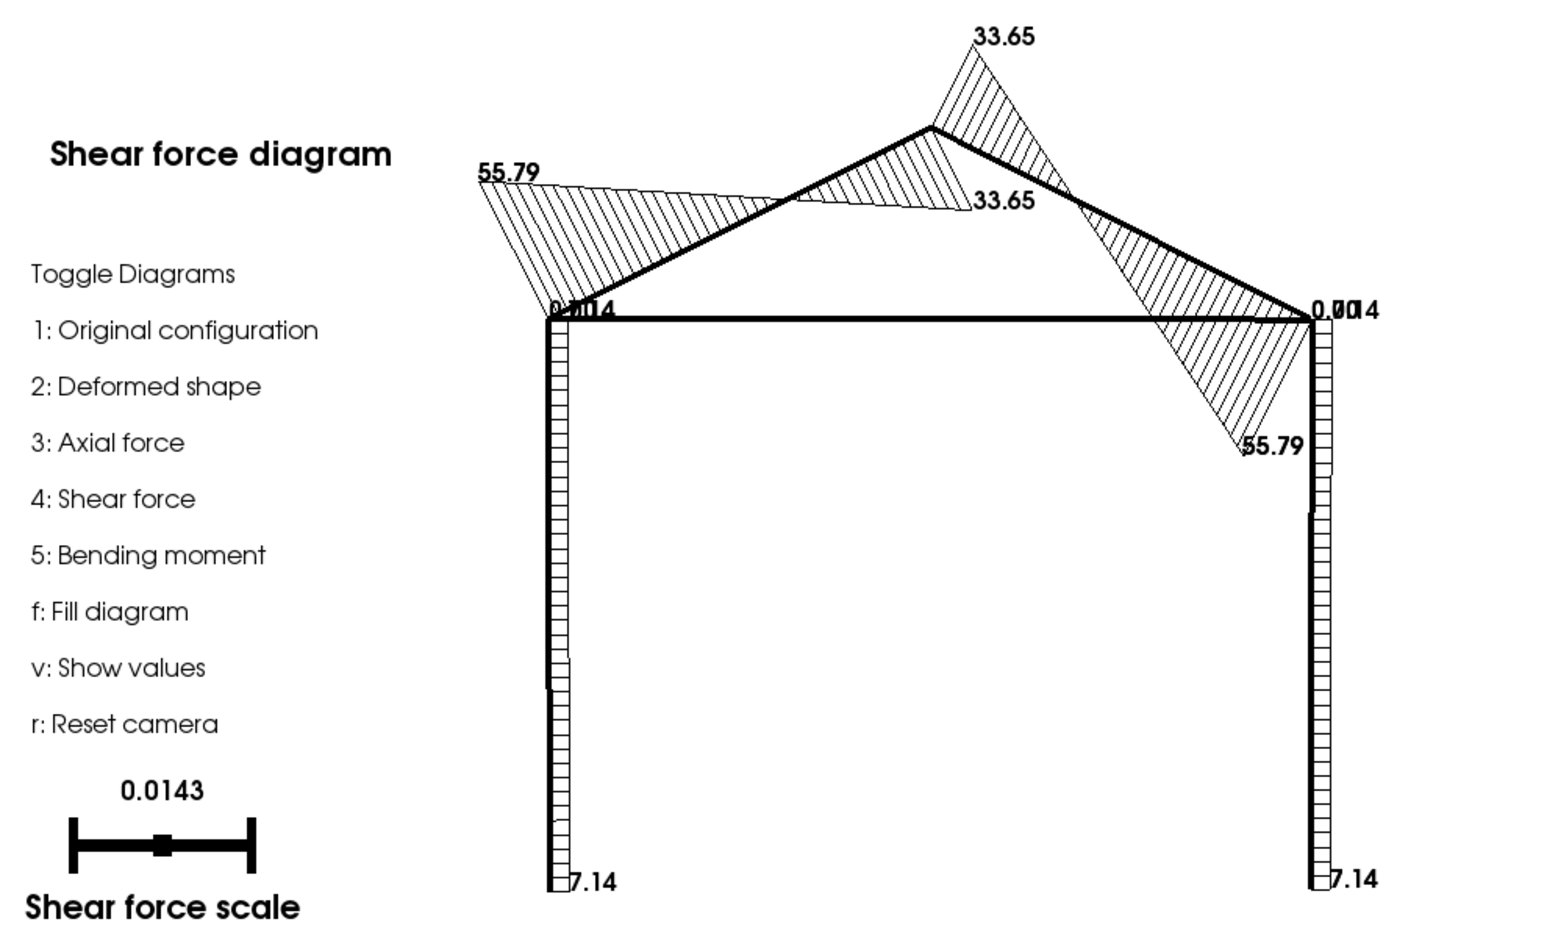
\includegraphics[width=\textwidth, keepaspectratio]{%
                     bm_figures/vtk_figures/bmsp04_shear.pdf}
    \centering
    \caption{Specialized Problem 4: Shear Force Diagram}
    \label{fig:bmsp04_shear}
\end{figure}
% Moment
\begin{figure}[!htb]
    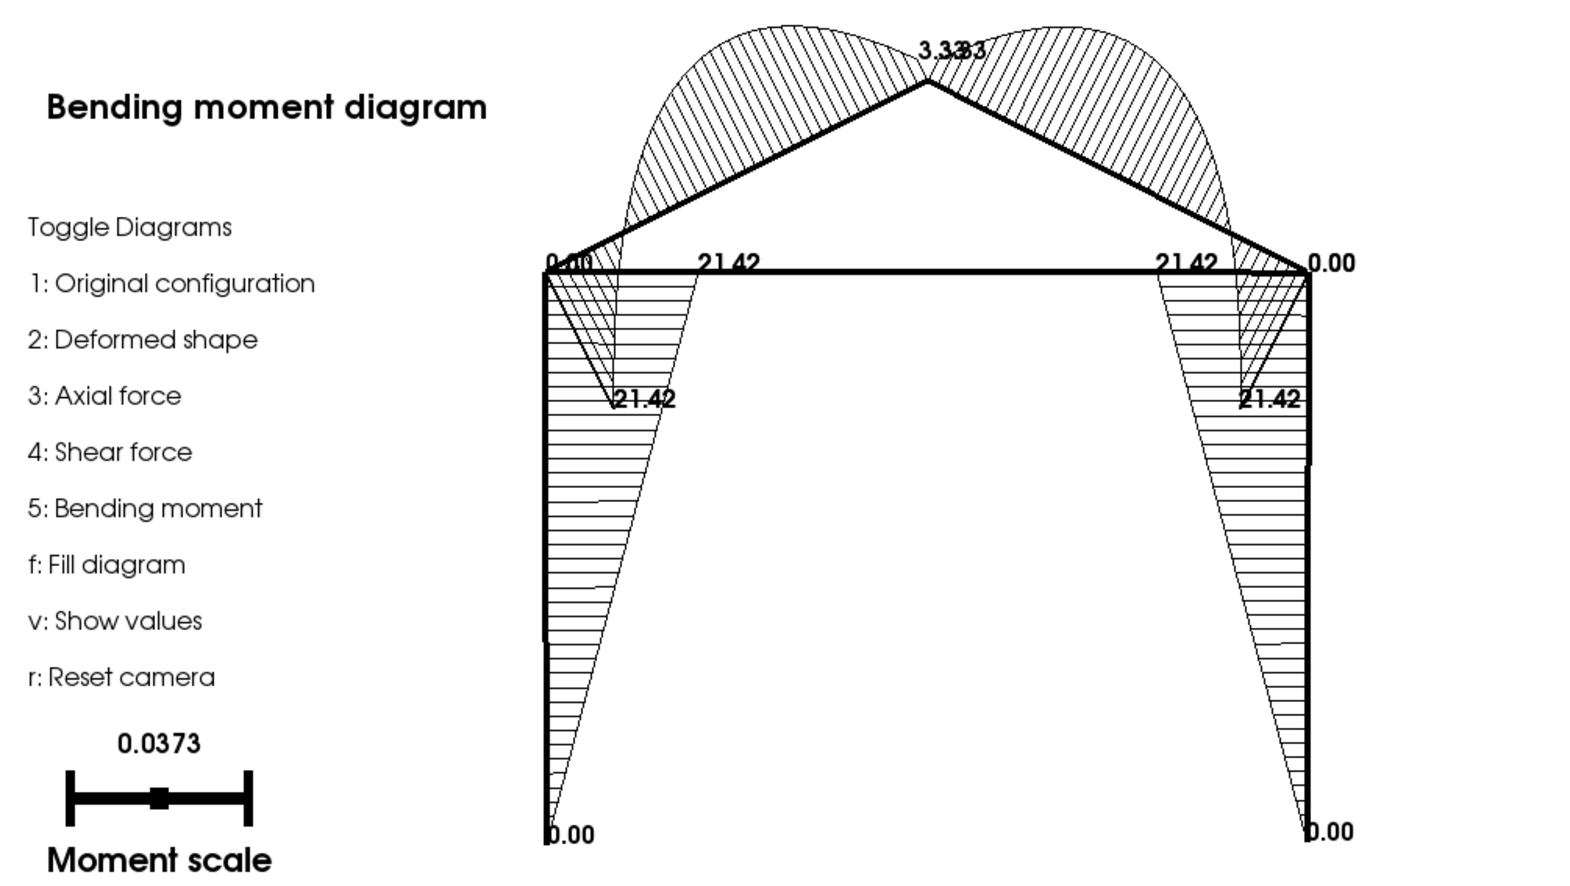
\includegraphics[width=\textwidth, keepaspectratio]{%
                     bm_figures/vtk_figures/bmsp04_moment.pdf}
    \centering
    \caption{Specialized Problem 4: Bending Moment Diagram}
    \label{fig:bmsp04_moment}
\end{figure}
% Error
\begin{table}[h!]
\centering
\begin{tabular}{ c| c c c }
    & Reference Value & Computed Value & \% RE \\ \hline \\
    $M_{2}=M_{4}$     & 0.21422E+02 & 0.21422E+02 & 0.0\% \\ \\
    $M_{3}$           & 0.33333E+01 & 0.33333E+01 & 0.0\% \\ \\
    $V_{1}=V_{5}$     & 0.10000E+03 & 0.10000E+03 & 0.0\% \\ \\
    $H_{5}=-H_{1}$    & 0.7141E+01 & 0.71413E+01 & 0.0\% \\ \\
\end{tabular}
\end{table}

